\titleformat{\chapter}[display]
{\normalfont\huge\bfseries}{Capítulo \thechapter}{0.5em}{\huge}
\titlespacing*{\chapter}{0pt}{-1.25cm}{25pt}
\chapter{Arquitectura e Implementacion}

En este capítulo se describirá la arquitectura de la aplicación, así como las tecnologías utilizadas para su implementación. 

\section{Arquitectura}

Se pueden categorizar los tres módulos (\textbf{Adquisición de datos}, \textbf{Procesamiento y análisis}, \textbf{Visualización y Presentación}) de la aplicación mencionados en el capitulo anterior en dos categorias principales:

\begin{itemize}
	\item \textbf{Adquisición de paquetes APRS:} En este módulo se encuentran los componentes encargados de la adquisición de paquetes APRS. Estos componentes se encargan de recibir los paquetes APRS, procesarlos y almacenarlos en la base de datos de la aplicación.
	
	\item \textbf{Aplicación web APRSINT:} En este módulo se encuentran los componentes encargados del análisis, la interpretación y la visualización, de los datos almacenados en la base de datos de la aplicación. Estos componentes se encargan de presentar la información de manera rápida y cómoda para el usuario. 
\end{itemize}

\section{Tecnologías utilizadas}

Como se ha mencionado anteriormente, uno de los objetivos de APRSINT es el de ser una solución accesible y fácil de usar. Para lograr este objetivo, se han seleccionado tecnologías ampliamente utilizadas y bien documentadas. A continuación se describen las tecnologías utilizadas en cada uno de los módulos de la aplicación.
\subsection{Raspberry Pi}

La Raspberry Pi es un \textit{Single board computer (SBC)} u ordenador de placa única desarrollada por la Fundación Raspberry Pi. Las raspberry pi son muy populares en el mundo de la informática y la electrónica por su bajo precio, reducido tamaño y su versatilidad.

\begin{itemize}
\item \textbf{Bajo precio:} La Raspberry es una opción económica para implementar desde prototipos hasta aplicaciones simples, lo que la hace muy accesible para una amplia gama de usuarios.
\item \textbf{Bajo Consumo Energético:} Su diseño de bajo consumo energético la hace ideal para aplicaciones que requieren funcionamiento continuo.
\item \textbf{Versatilidad:} La Raspberry Pi 4 es altamente versátil y puede adaptarse a una variedad de casos de uso, desde servidores ligeros hasta placas de desarrollo para robótica y automatización. 
\end{itemize}
Se ha seleccionado la Raspberry Pi 4b\footnote{Cuando se comenzó el proyecto todavía no se habia lanzado la versión 5.} de 8GB de memoria ram como plataforma de hardware para la implementación de la solución, debido a sus características y capacidades.

\subsection{Disco duro ssd}
Los discos duros de estado sólido (SSD) son una alternativa a los discos duros tradicionales (HDD) que ofrecen una mayor velocidad de lectura y escritura, menor consumo energético y mayor durabilidad. Se ha seleccionado un disco duro SSD de 250GB que se haya conectado a la raspberry-pi para almacenar el gran volumen de datos que consume y genera la aplicacion a su velocidad y fiabilidad.

\subsection{Python}
Python es un lenguaje de programación interpretado, de alto nivel y de propósito general. Es ampliamente utilizado en el desarrollo de aplicaciones web, científicas y de análisis de datos debido a su simplicidad, flexibilidad y facilidad de uso. Se ha seleccionado Python como lenguaje de programación principal para la implementación de la solución debido a la gran versatilidad que ofrece y sobretodo por la existencia de extensas librerias de visualización y manejo de grandes volumenes de datos.

\subsection{Dash}
Dash es un framework de Python creado por plotly para la creación de aplicaciones web interactivas y visualizaciones de datos. Dash permite crear aplicaciones web interactivas y visualizaciones de datos atractivas utilizando Python como lenguaje de programación. Dash esta construido encima de React Se ha seleccionado Dash como framework para la implementación de la interfaz web de la aplicación debido a su facilidad de uso y a la gran cantidad de funcionalidades que ofrece. Dash está escrito encima de Plotly.js, React y Flask lo que permite una gran capacidad de customizacion.

\begin{itemize}
	\item \textbf{Interactividad:} Dash permite crear aplicaciones web altamente interactivas, lo que facilita la exploración de datos y la toma de decisiones.
	\item \textbf{Flexibilidad:} Su arquitectura modular y su amplia gama de componentes permiten la creación de aplicaciones web personalizadas y adaptadas a las necesidades específicas del usuario.
	\item \textbf{Integración con Plotly:} Al estar desarrollado por Plotly, Dash ofrece una integración perfecta con las capacidades de visualización de datos de Plotly, lo que permite crear gráficos y visualizaciones muy atractivas.
\end{itemize}

Para crear la aplicación web se consideraron algunas alternativas como Django, Streamlit y PowerBI, sin embargo, Dash fue la opción escogida debido a su extensa capacidad de customizacion y personalizacion de la que carecian las demás opciones.

\subsection{Cosmograph JS}

Cosmograph es una libreria de JavaScript enfocada en la visualización de grandes grafos y redes complejas en aplicaciones web. Permite representar de manera interactiva relaciones entre entidades, facilitando la comprensión y el análisis de datos estructurados.

\begin{itemize}
\item \textbf{Visualización de Grafos:} Cosmograph ofrece herramientas avanzadas para la representación visual de grafos como lineas temporales, histogramas y búsquedas de nodos, una mayor comprensión y capacidad de análisis de la información.

\item \textbf{Rendimiento:} Cosmograph a diferencia de otras librerias más populares como Sigma JS transfiere todos los cálculos de posiciones de los nodos y aristas así como la representación gráfica de este a la GPU. Esto permite la visualización de grafos con miles de nodos y aristas sin afectar el rendimiento de la aplicación.

\item \textbf{Personalización:} Ofrece opciones de personalización para adaptar la apariencia y el comportamiento de los nodos y aristas según las necesidades específicas del usuario.

\end{itemize}

Después de una gran cantidad de pruebas y tras considerar muchas alternativas como Sigma Js, CytoScape y networkx, se acabó eligiendo Cosmograph sobre todo por su rendimiento.

\subsection{PostgreSQL}

PostgreSQL es un sistema de gestión de bases de datos relacional de código abierto y potente, conocido por su fiabilidad, robustez y capacidad para manejar grandes volúmenes de datos. Ofrece una amplia gama de características avanzadas que lo hacen adecuado para aplicaciones web y empresariales exigentes.

\begin{itemize}
\item \textbf{Fiabilidad y Robustez:} PostgreSQL es conocido por su alta fiabilidad y capacidad para manejar grandes cargas de trabajo sin sacrificar el rendimiento.
\item \textbf{Escalabilidad:} Es altamente escalable y puede manejar grandes volúmenes de datos y transacciones concurrentes sin problemas.
\item \textbf{Funcionalidades Avanzadas:} Ofrece una amplia gama de funcionalidades avanzadas, como soporte para transacciones ACID, vistas materializadas, procedimientos almacenados y Full Text Search (búsqueda de indizada).
\item \textbf{Almacenamiento de datos semiestructurados:} PostgreSQL es capaz de almacenar y manipular datos no estructurados como JSON de manera eficiente, lo que lo hace adecuado para aplicaciones que requieren almacenamiento de datos semiestructurados.
\item \textbf{Rendimiento:} PostgreSQL ofrece un rendimiento sólido, especialmente en entornos de alta concurrencia y cargas de trabajo intensivas.
\end{itemize}

La elección de PostgreSQL como sistema de gestion de bases de datos se debió a su robustez, facilidad de uso y a la gran cantidad de funcionalidades que ofrece.

\subsection{Sqlalchemy}
\subsection{aprslib}
\subsection{AWS}
\subsection{Supervisord}
\subsection{Pandas}
\subsection{Airflow}


\begin{figure}[h]
    \centering
    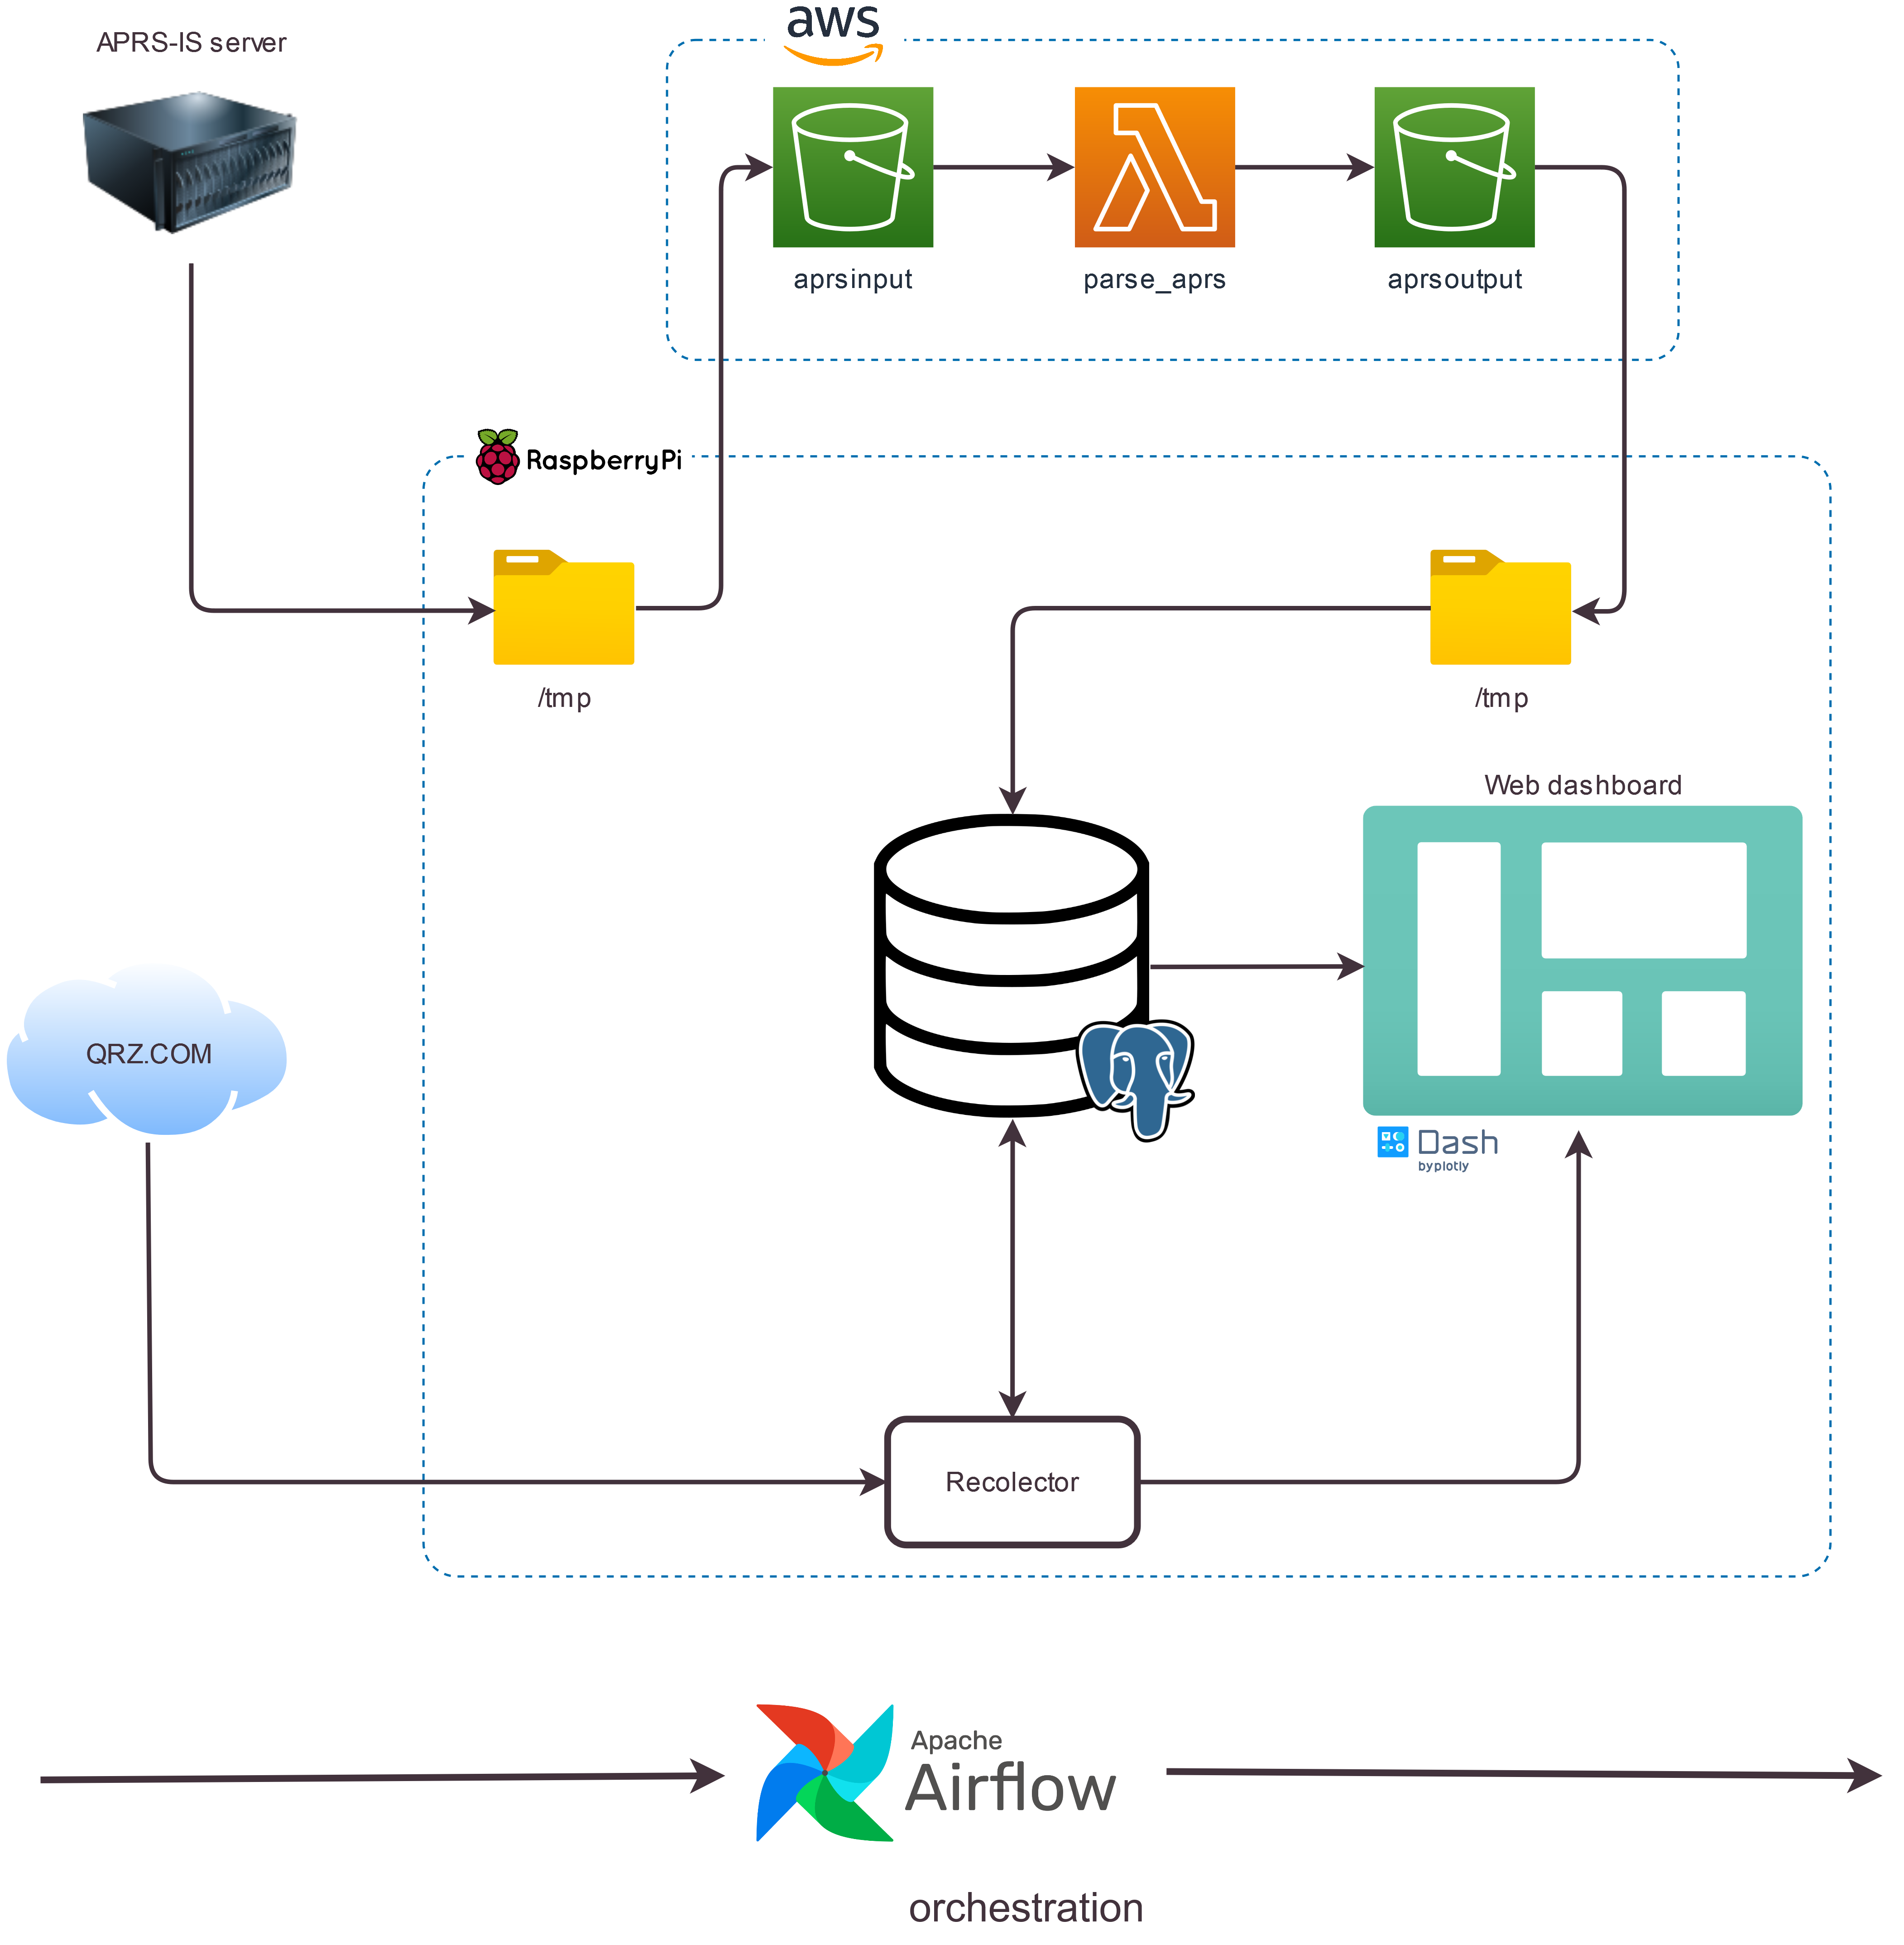
\includegraphics[width=0.85\textwidth]{./Chapter_4/cloud_arch.png}
    \caption{Estructura base de la aplicación.}
    \label{fig:cloud-architecture}
\end{figure}